\documentclass{beamer}
\usepackage{amsfonts,amsmath,oldgerm,multimedia}
\usepackage[italian]{babel}
\usetheme{sintef}

\newcommand{\testcolor}[1]{\colorbox{#1}{\textcolor{#1}{test}}~\texttt{#1}}

\usefonttheme[onlymath]{serif}

\titlebackground*{images/default}

\newcommand{\hrefcol}[2]{\textcolor{cyan}{\href{#1}{#2}}}

\title{Sistemi di correzione della stima della posa di un AGV}
\subtitle{Gruppo M}
\author{Pietro Agnelli, Matteo Berardi, Riccardo Valtorta}
\date{Laboratorio di misure industriali}

\begin{document}
\maketitle

\begin{frame}{Contesto e obiettivi}
\begin{itemize}
\item Il problema che abbiamo affrontato nel corso del progetto è stato quello di sviluppare metodi per la stima della posa di un veicolo a guida autonoma (AGV).
\item Il veicolo deve operare in ambiente agricolo, all'interno di filari.
\item Lo strumento di misura impiegato per la stima della posa è una telecamera \textbf{Intel realsense T265}, che monta, oltre a due ottiche \emph{fisheye}, un'unità inerziale \textbf{Bosh BMI055}.
\item Gli algoritmi scelti per la correzione della stima della posizione sono:
\begin{itemize}
    \item teorema del limite centrale (CLT),
    \item Bayes,
    \item filtro di Kalman.
\end{itemize}
% TODO: inserire tabella con dati sensore
\begin{figure}
    \centering
    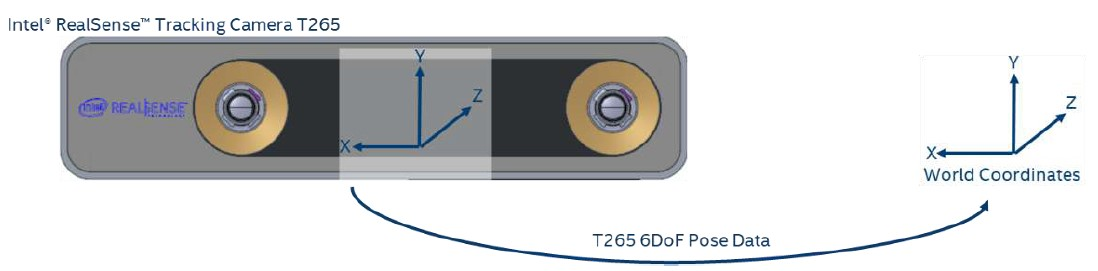
\includegraphics[height=2.3cm]{images/t265.jpg}
    \caption{Sistema di coordinate del dispositivo realsense t265}
    \label{fig:t265coord}
\end{figure}
\end{itemize}
\end{frame}

\begin{frame}{Roadmap}
\begin{columns}
\begin{column}{0.6\textwidth}
Lo svolgimento del progetto si è articolato nelle seguenti fasi:
\begin{enumerate}
    \item Stima dell'incertezza associata a misurazioni con marker \emph{ArUco}
    \item Stima dell'incertezza associata alle misurazioni odometriche
    \item Studio e implementazione degli algoritmi di sensor fusion
    \item Applicazione degli algoritmi ad un caso reale
\end{enumerate}
\end{column}
\begin{column}{0.4\textwidth}
    \begin{figure}
        \centering
        
\includegraphics[width=0.7\textwidth]{images/marker23.png}
        \caption{un marker ArUco.}
        \label{fig:markerArUco}
    \end{figure}
\end{column}
\end{columns}
\end{frame}

\begin{frame}{Stima dell'incertezza associata ai marker ArUco}
\framesubtitle{Setup sperimentale e protocollo}
\begin{columns}
\begin{column}{0.6\textwidth}
Abbiamo eseguito 2 prove percorrendo la guida per l'intera lunghezza, effettuando un'andata e un ritorno, in ciascuna direzione:
    \begin{itemize}
        \item Traslazione della camera lungo l'asse $x$
        \item Traslazione della camera lungo l'asse $z$
        \item Traslazione della camera verso il marker con un angolo di inclinazione $\theta = 30°,45°,60°$ rispetto all'asse $x$
    \end{itemize}
Successivamente abbiamo stimato l'incertezza associata alle misure attraverso una regressione ai minimi quadrati.
\end{column}
\begin{column}{0.4\textwidth}
    \begin{figure}
        \centering
        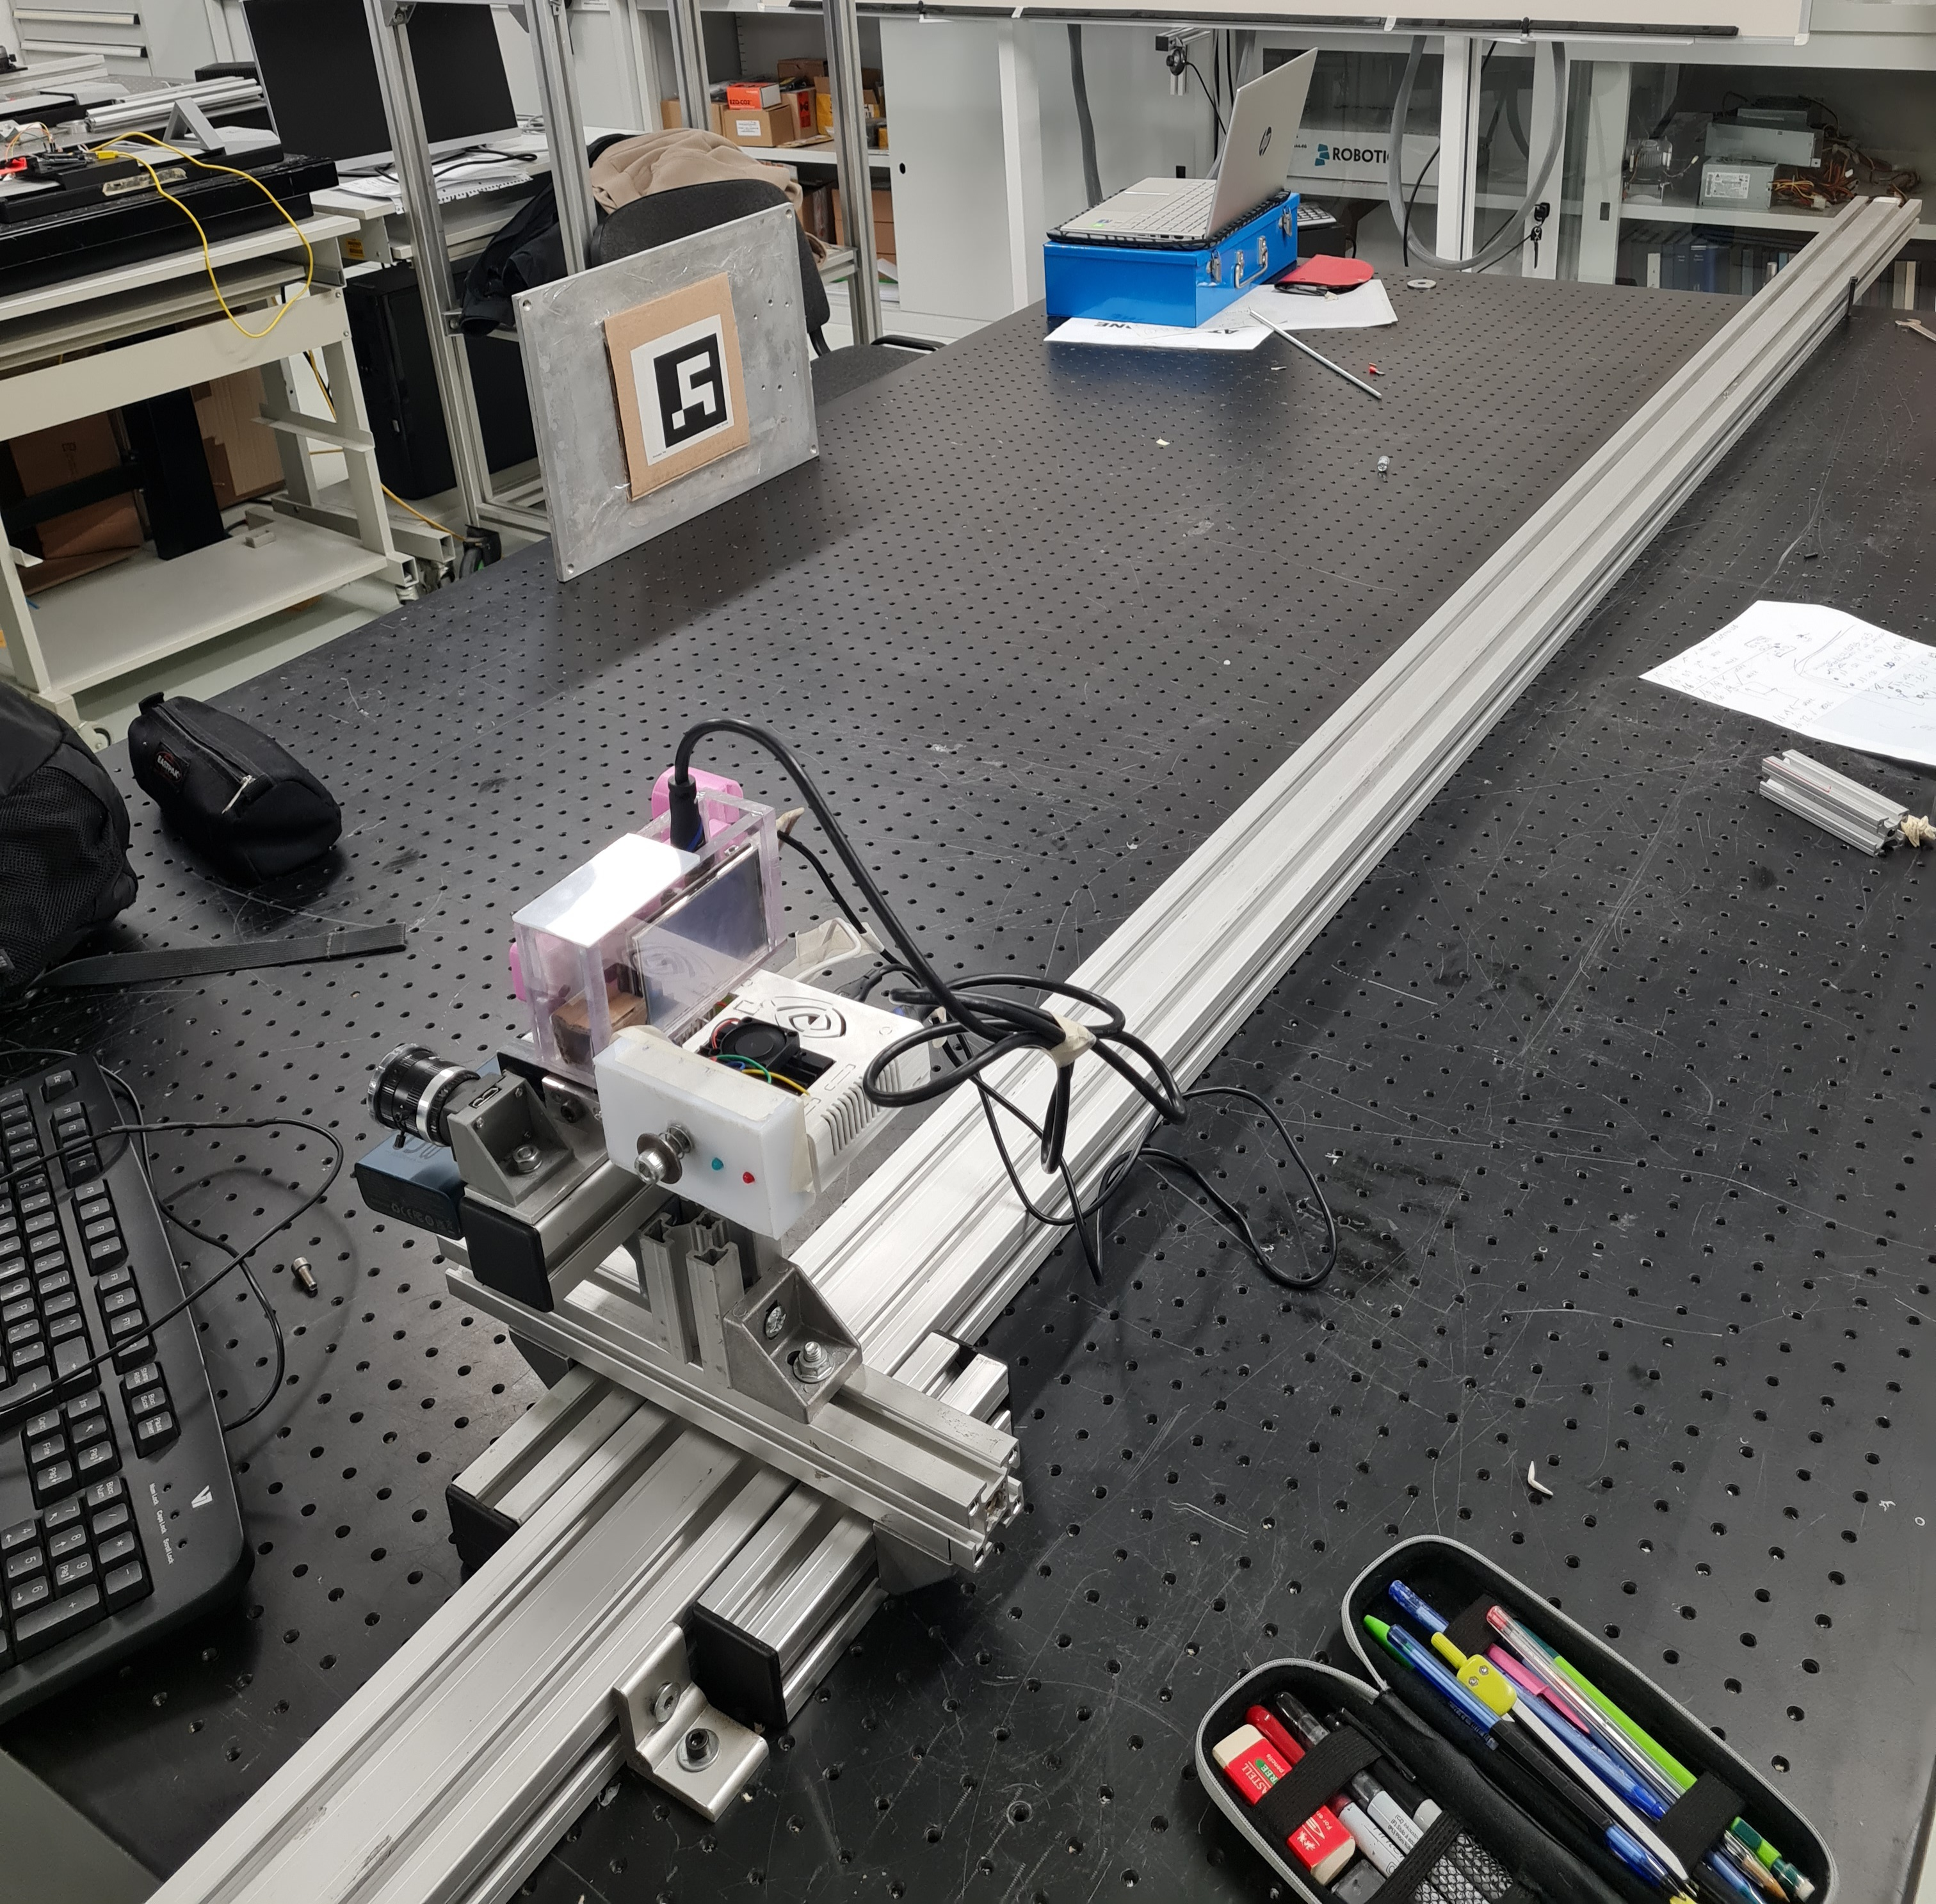
\includegraphics[width=0.7\textwidth]{images/setupArUco.jpg}
        \caption{Setup per la misura dell'incertezza associata al marker nella misura della posizione lungo l'asse $z$.}
        \label{fig:setupArUco}
    \end{figure}
\end{column}
\end{columns}
\end{frame}

\begin{frame}{Stima dell'incertezza associata ai marker ArUco}
\framesubtitle{Risultati della stima}
\begin{columns}
    \begin{column}{0.8\textwidth}
        \begin{figure}
            \centering
            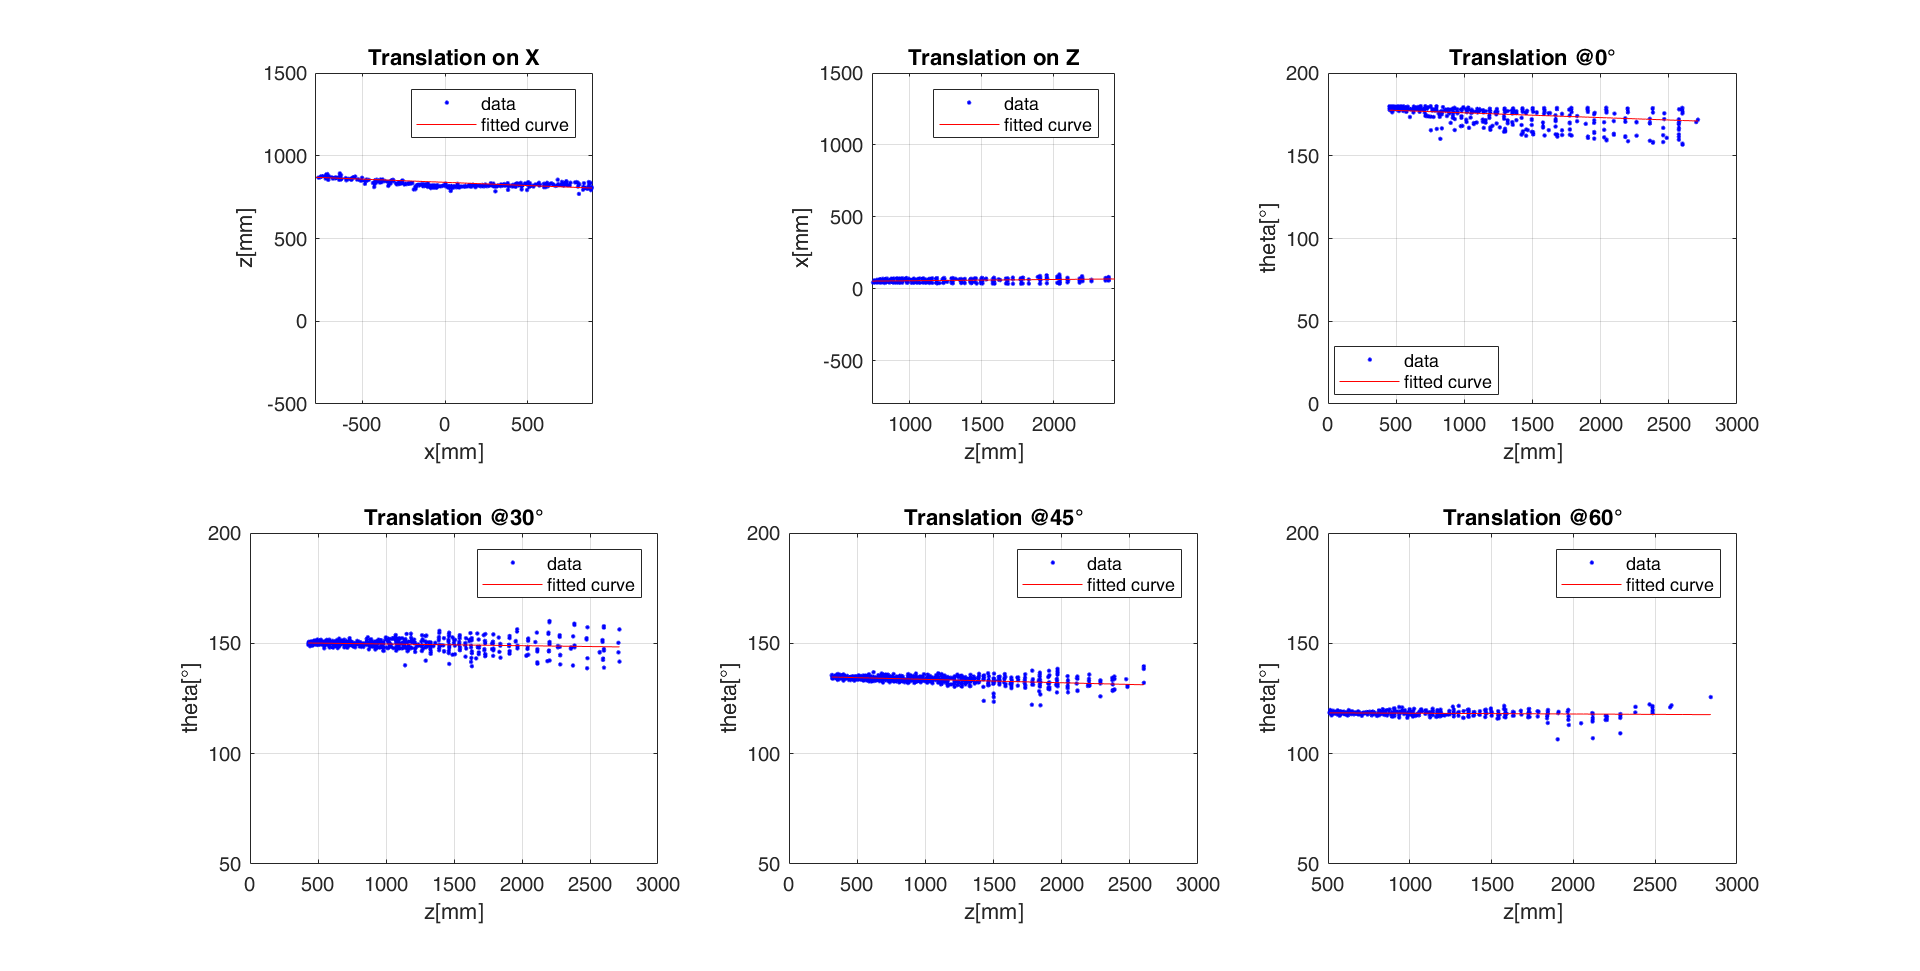
\includegraphics[width=\textwidth]{images/arucoreg.png}
            \label{fig:arucoreg}
        \end{figure}
    \end{column}
    \begin{column}{0.2\textwidth}
        \begin{table}[h]
            \centering
            \begin{tabular}{|c|c|c|}
                \hline
                $\sigma_x$ [$mm$] & $13$\\
                \hline
                $\sigma_z$ [$mm$] & $19$\\ 
                \hline
                $\sigma_{\theta}$ [$^{\circ}$] &$5.7$\\
                \hline
            \end{tabular}
            \caption{Incertezze sulle misure dei marker ArUco.}
            \label{tab:uaruco}
        \end{table}
    \end{column}
\end{columns}
\end{frame}

\begin{frame}{Stima dell'incertezza associata alle misure odometriche}
\framesubtitle{Approccio generale}
\begin{itemize}
    \item Stima più complessa in quanto si tratta di un'incertezza \emph{incrementale}
    \item Abbiamo valutato due diversi approcci:
    \begin{enumerate}
        \item calcolo mediante propagazione dell'incertezza:
        \begin{equation}
            x_n =x_{n-1}+\Delta x  \cos{(\theta_{n-1})} \rightarrow
        \end{equation}
        \begin{equation}
        \rightarrow\sigma_{x_n}^2 = \sigma_{x_{n-1}}^2 + \sigma_{\Delta x}^2 \cos{(\theta_{n-1})}^2 + \sigma_{\theta_{n-1}}^2 \Delta x ^2 \sin{(\theta_{n-1})}^2
        \label{eq:prop}
\end{equation}
\begin{equation}
    \sigma_{\theta_{n}}^2 = \sigma_{\theta_{n-1}}^2 + \sigma_{\omega}^2 \delta t^2
    \label{eq:angleprop}
\end{equation}
        \item stima mediante modello:
\begin{equation}
    y = \beta_0 + \beta_{1}p_{x} + \beta_{2}p_{z} + \beta_{3}v_{x} + \beta_{4}v_{z} + \beta_{5}\theta
    \label{eq:model}
\end{equation}
\end{enumerate}
\end{itemize}
\end{frame}

\begin{frame}{Stima dell'incertezza associata alle misure odometriche}
\framesubtitle{Test in posizione statica}
\begin{columns}
    \begin{column}{0.6\textwidth}
    \begin{figure}
            \centering
            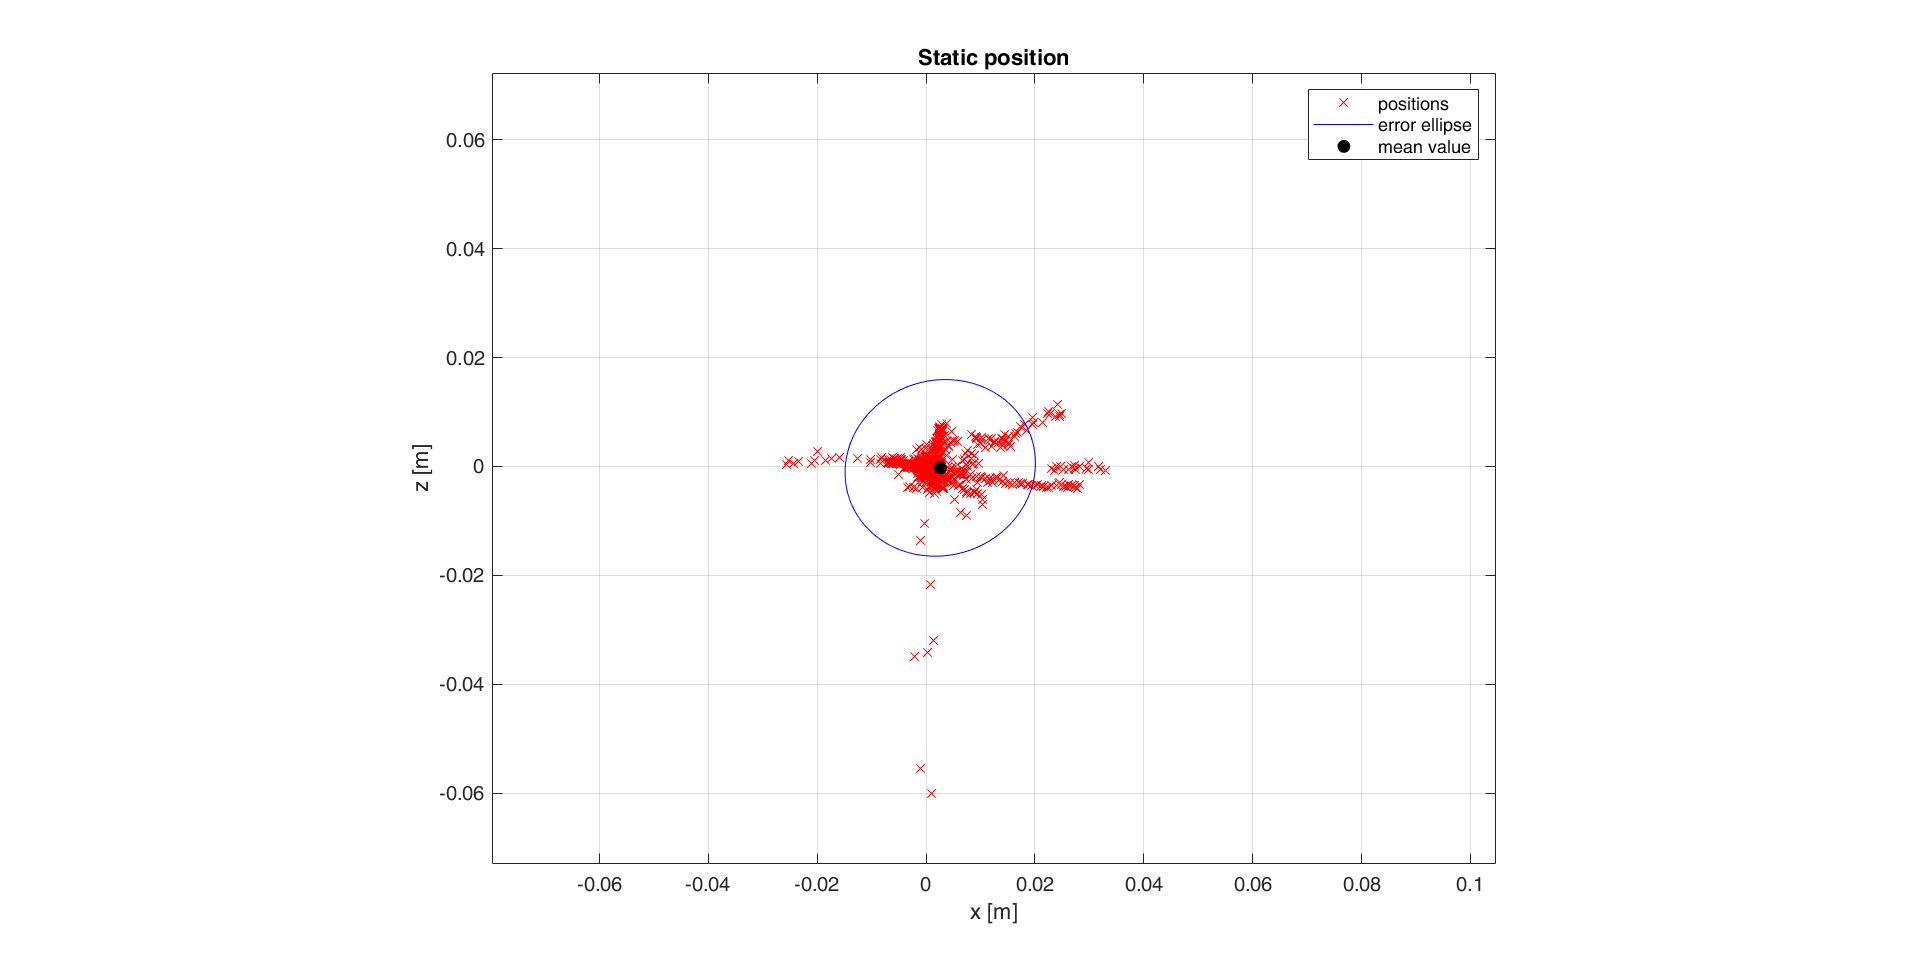
\includegraphics[width=10cm]{images/static.png}
            \label{fig:staticpos}
        \end{figure}
        
    \end{column}
    \begin{column}{0.4\textwidth}
        Abbiamo eseguito una prova per determinare l'incertezza sulla stima di una posizione statica:
        \begin{enumerate}
            \item avvio dell'acquisizione
            \item attesa $5s$
            \item arresto dell'acquisizione
        \end{enumerate}
        Sono state eseguite 10 \emph{runs}.
    \end{column}
\end{columns}
\end{frame}

\begin{frame}{Stima dell'incertezza associata alle misure odometriche}
\framesubtitle{Test a distanze e angoli noti}
Abbiamo eseguito una prova per determinare l'incertezza sulla stima della posizione incrementale:
        \begin{enumerate}
            \item avvio dell'acquisizione
            \item attesa $5s$
            \item spostamento verso la posizione di destinazione
            \item attesa $5s$
            \item arresto dell'acquisizione
        \end{enumerate}
        Sono state eseguite 10 \emph{runs} per distanze da $500\ mm$ a $2000\ mm$, a intervalli di $500\ mm$ in direzione $x$ e $z$ e altrettante prove per angoli $\theta=30^{\circ},45^{\circ},60^{\circ},90^{\circ}$.
        Il setup per le prove lineari è analogo a quello utilizzato per la stima dell'incertezza associata ai marker, con l'aggiunta di fermi posti alle distanze di riferimento. Le prove angolari hanno seguito lo stesso meccanismo, usando un'asta incernierata ad un'estremità come guida.
\end{frame}

\begin{frame}{Stima dell'incertezza associata alle misure odometriche}
\framesubtitle{Test a distanze e angoli noti (risultati)}
\begin{figure}
    \centering
    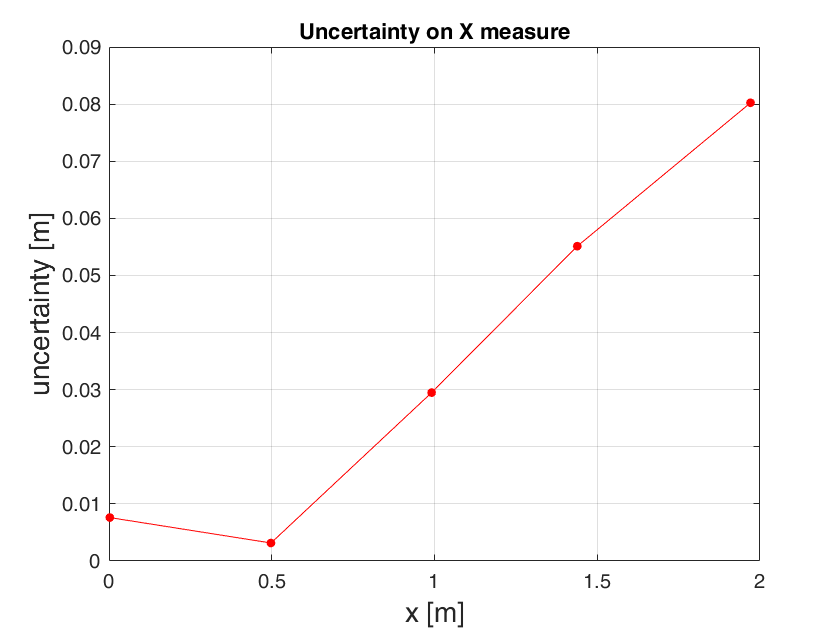
\includegraphics[width=0.3\textwidth]{images/xexpu.png}
    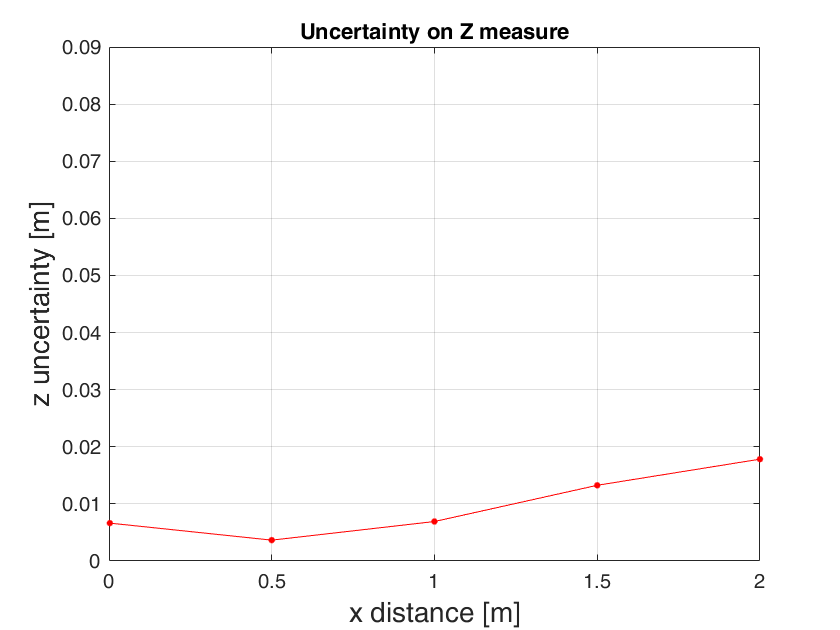
\includegraphics[width=0.3\textwidth]{images/zexpu.png}
    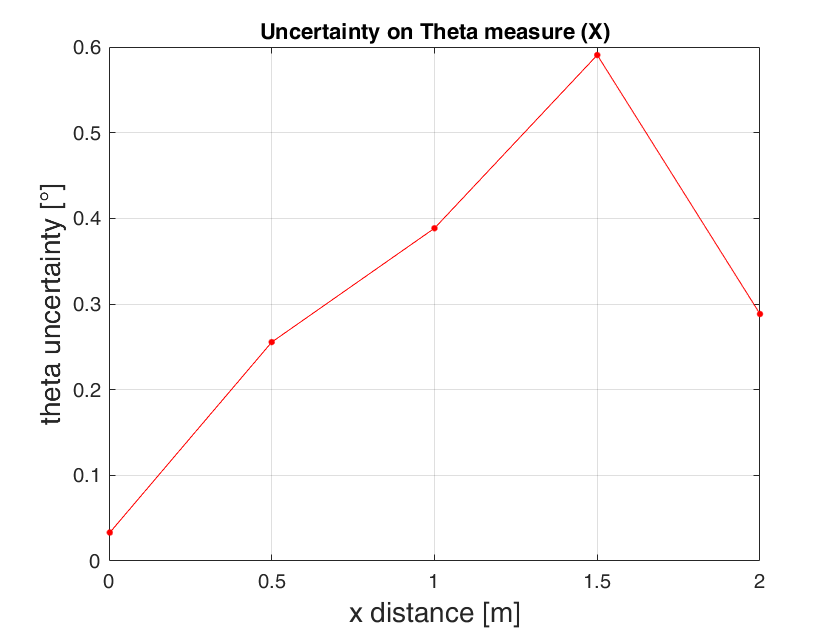
\includegraphics[width=0.3\textwidth]{images/thetaexpu.png}
\end{figure}
\begin{table}[h]
    \centering
    \begin{tabular}{|c|c|c|c|c|c|}
    \hline
       $x$ [$mm$]          & $0$ & $500$ & $1000$ & $1500$ & $2000$\\
    \hline
        $\sigma_x$ [$mm$]&  $7.7$ & $3.2$ & $30$ & $55$ & $80$\\
        $\sigma_z$ [$mm$]&  $6.6$ & $3.7$ & $6.9$ & $13$ & $18$\\
        $\sigma_{\theta} [$°$]$ & $0.033$ & $0.26$ & $0.38$ & $0.59$ & $0.29$\\
    \hline
    \end{tabular}
    \caption{Incertezze sulle misure odometriche al variare della distanza percorsa.}
    \label{tab:uncertainties}
\end{table}
\end{frame}

\begin{frame}{Stima dell'incertezza associata alle misure odometriche}
\framesubtitle{Propagazione dell'incertezza}
\begin{columns}
    \begin{column}{0.6\textwidth}
    \begin{figure}
            \centering
            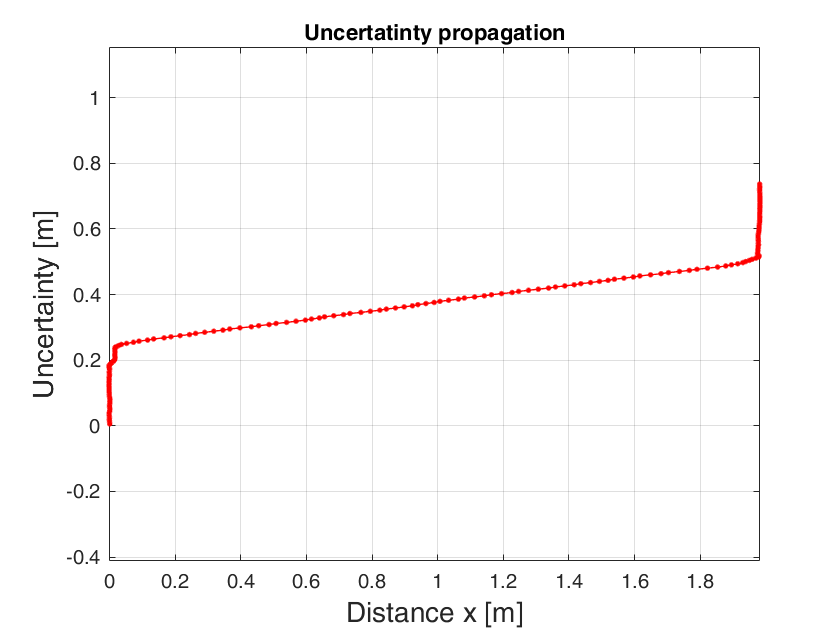
\includegraphics[width=8cm]{images/propagation.png}
            \label{fig:staticpos}
        \end{figure}
        
    \end{column}
    \begin{column}{0.4\textwidth}
    \begin{itemize}
        \item La propagazione teorica dell'incertezza non risulta coerente con i dati sperimentali rilevati.
        \item L'algoritmo di elaborazione interno alla camera non è pubblicamente noto.
        \begin{table}[]
            \centering
            \begin{tabular}{|c |c|}
            \hline
               $\sigma_{gyro}$  & $1^{\circ}/s$ \\
               \hline
               $\sigma_{acc}$ & $70\ mm/s^{2}$\\
               \hline
            \end{tabular}
            \caption{Dati di incertezza BOSH BMI055, in condizioni standard.}
        \end{table}
    \end{itemize}
    \end{column}
\end{columns}
\end{frame}

\begin{frame}{Stima dell'incertezza associata alle misure odometriche}
\framesubtitle{Stima con modello}
\begin{columns}
    \begin{column}{0.6\textwidth}
    \begin{figure}
            \centering
            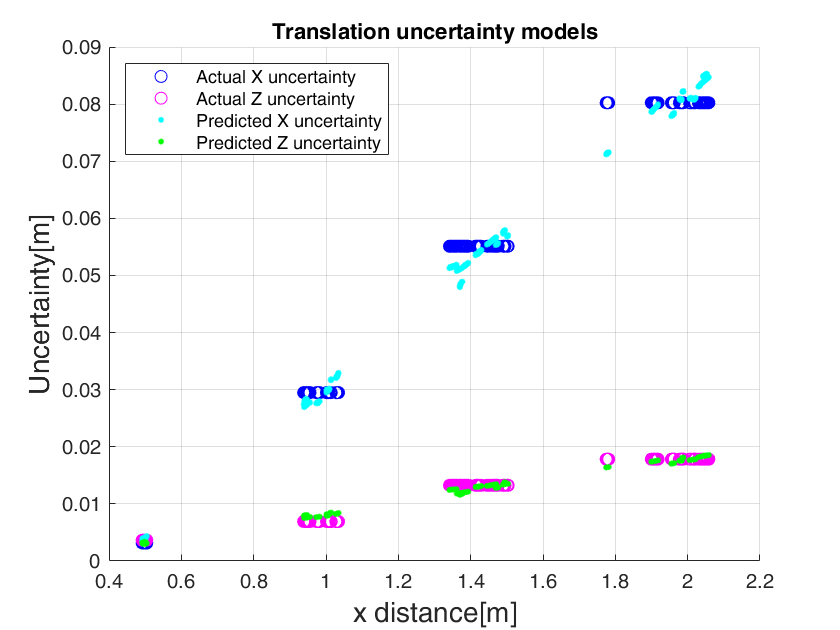
\includegraphics[width=8cm]{images/model.png}
            \label{fig:staticpos}
        \end{figure}
    \end{column}
    \begin{column}{0.4\textwidth}
    \begin{itemize}
        \item Modello tiene in considerazione diverse variabili:
        \begin{table}[]
            \centering
            \begin{tabular}{|c |c|}
            \hline
               $E_{x}$  & $0.19\%$ \\
               \hline
               $E_{z}$ & $0.057\%$\\
               \hline
               $E_{\theta}$ & $7.0\%$\\
               \hline
            \end{tabular}
            \caption{Errore relativo del modello nella stima dell'incertezza incrementale.}
        \end{table}
        \item ottiene prestazioni nettamente migliori nella modellizzazione del sensore.
    \end{itemize}
\end{column}
\end{columns}
\end{frame}

\begin{frame}{Algoritmi di sensor fusion}
\framesubtitle{Teorema del limite centrale (CLT)}
\begin{columns}
    \begin{column}{0.6\textwidth}
    \begin{figure}
        \centering
        \includegraphics[height=5cm]{images/clt.pdf}
        \caption{Diagramma di flusso dell'implementazione del clt.}
    \end{figure}
    \end{column}
    \begin{column}{0.4\textwidth}
    $$ x_{f} = \sum_{i=1}^{n}(z_{i}w_{i})$$
    $$ \sigma_{f} = \frac{1}{\sum_{i=1}^{n}(\sigma_{i}^{-2})} $$
    $$ w_{i} = \sigma_{i}^{-2}\sum_{i=1}^{n}(\sigma_{i}^{-2})$$
    $$\sum_{i=1}^{n} w_i = 1$$
\end{column}
\end{columns}
\end{frame}

\begin{frame}{Algoritmi di sensor fusion}
\framesubtitle{Teorema del limite centrale (CLT)-risultati}
    \begin{figure}
        \centering
        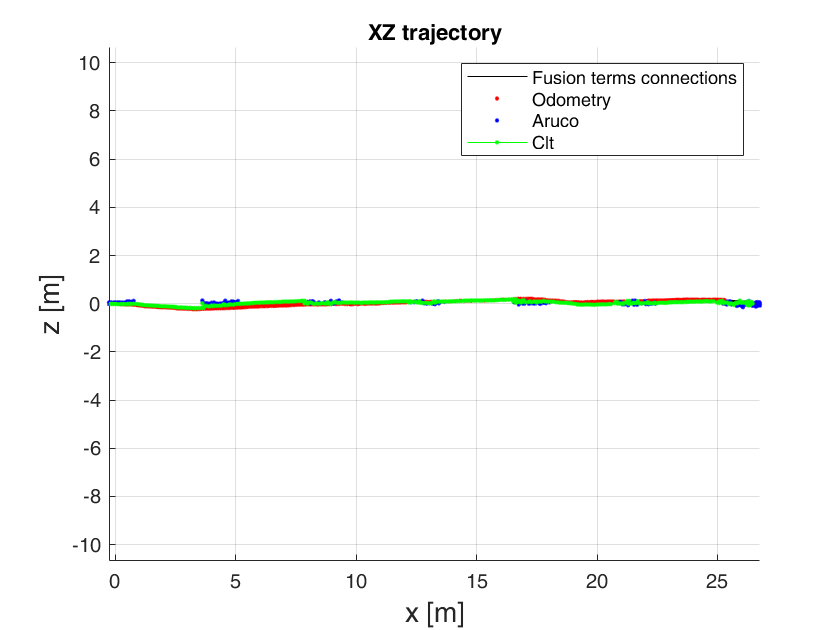
\includegraphics[width=.4\textwidth]{images/cltexpaxeq.png}
        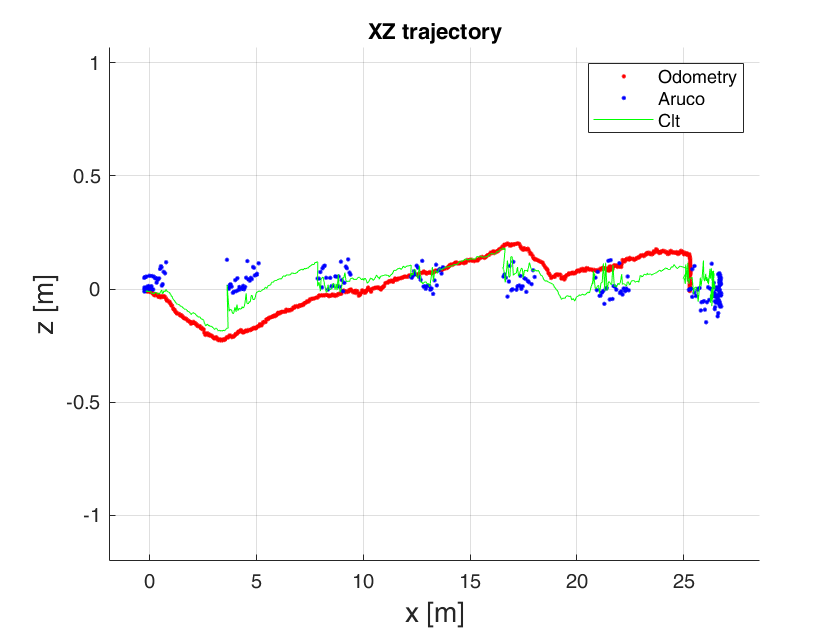
\includegraphics[width=.4\textwidth]{images/cltexp.png}
        \caption{Grafico dei risultati della fusione, su due scale differenti.}
    \end{figure}
\end{frame}

\begin{frame}{Algoritmi di sensor fusion}
\framesubtitle{Teorema del limite centrale (CLT)-risultati}
    \begin{figure}
        \centering
        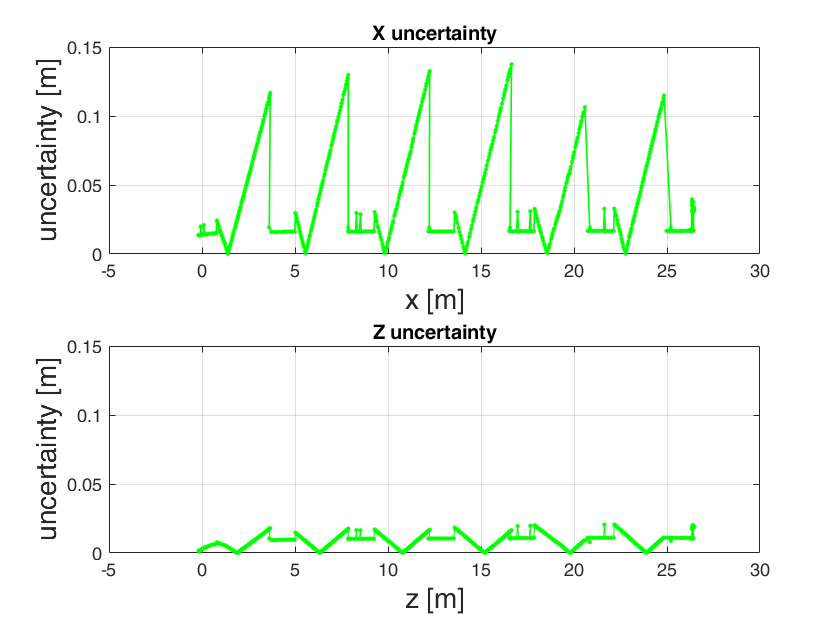
\includegraphics[width=.4\textwidth]{images/fusedunc.png}
        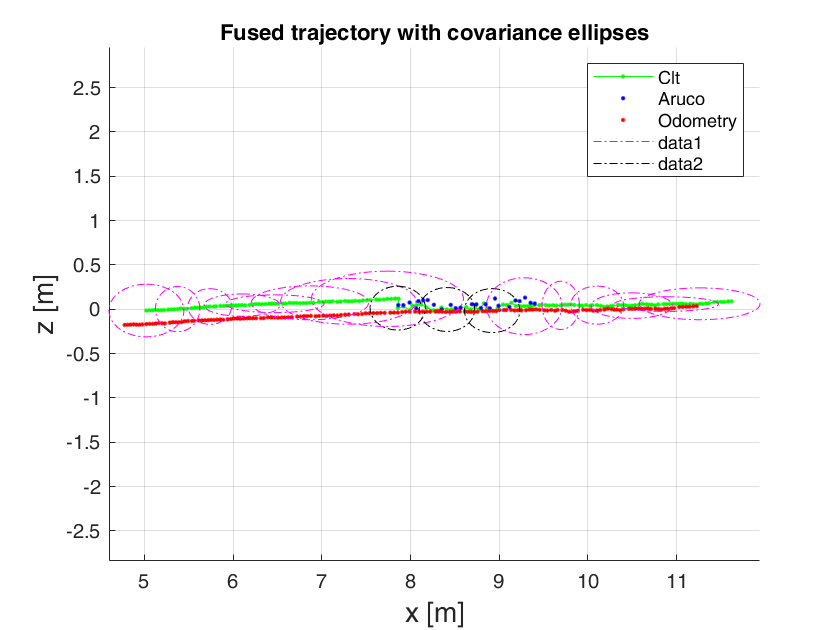
\includegraphics[width=.4\textwidth]{images/covelipses.png}
        \caption{Influenza della fusione sull'incertezza di misura.}
    \end{figure}
\end{frame}

\begin{frame}{Algoritmi di sensor fusion}
\framesubtitle{Filtro di Kalman}
    \begin{figure}
        \centering
        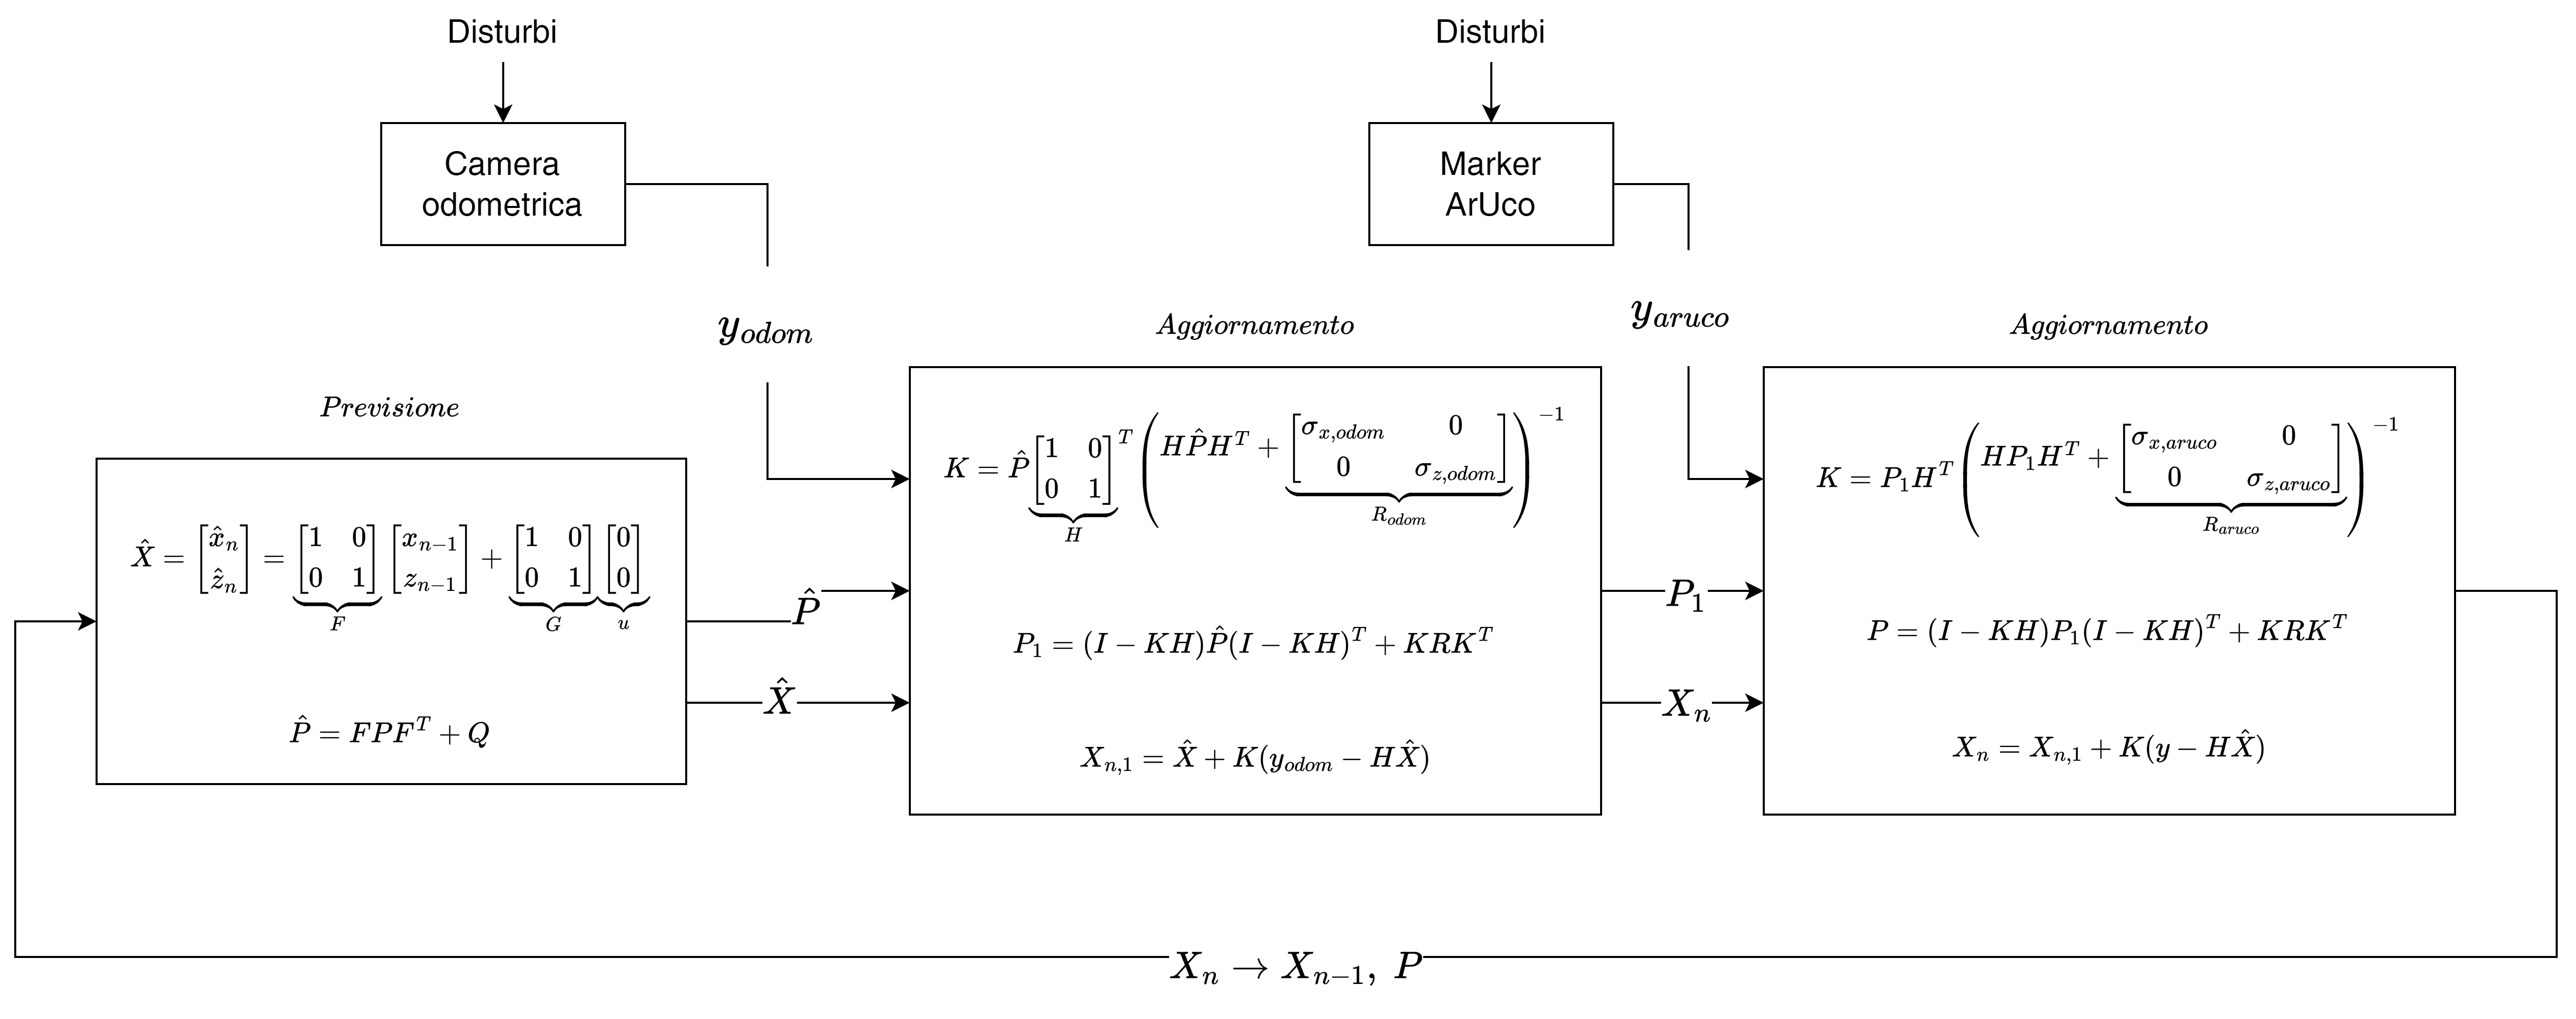
\includegraphics[width =\textwidth]{images/kfdiagram.png}
    \end{figure}
\end{frame}

\begin{frame}{Algoritmi di sensor fusion}
\framesubtitle{Filtro di Kalman-risultati}
    \begin{figure}
        \centering
        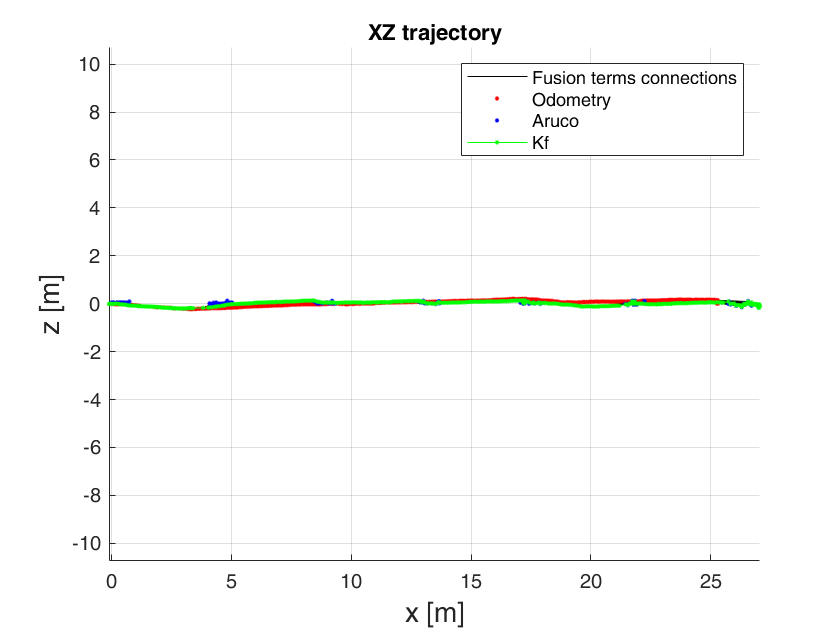
\includegraphics[width=.4\textwidth]{images/kfexpaxeq.png}
        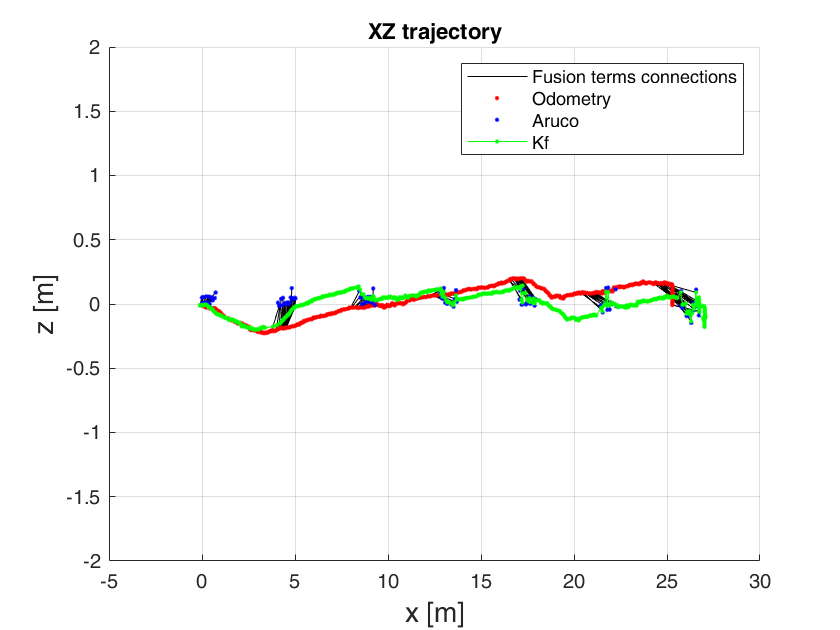
\includegraphics[width=.4\textwidth]{images/kfexp.png}
        \caption{Grafico dei risultati della fusione, su due scale differenti.}
    \end{figure}
\end{frame}

\begin{frame}{Algoritmi di sensor fusion}
\framesubtitle{Teorema di Bayes}
% TODO da completare questa slide
\begin{columns}
    \begin{column}{0.6\textwidth}
    \begin{figure}
        \centering
        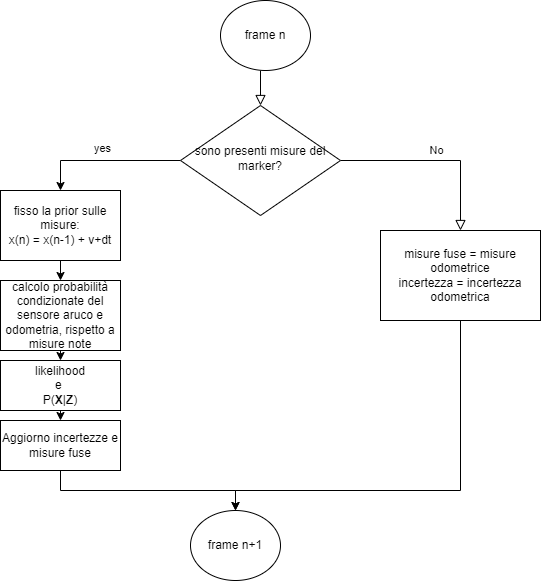
\includegraphics[height=5cm]{images/flowchart BAyes.png}
        \caption{Diagramma di flusso dell'implementazione di bayes.}
    \end{figure}
    \end{column}
    \begin{column}{0.4\textwidth}
    teorema: $P(X|Z)P(Z) = P(Z|X)P(X)$
    $$P(Z|X)=\frac{1}{\sqrt{2\pi}\sigma_{Z}} e^{-\frac{1}{2}\frac{(X-realmeasure)^{2}}{\sigma_{Z}}}$$
    $$P(X|X_{t-1}): prior$$
    $$prior_{x}: x(t) = x(t-1) + v*dt, \sigma_{x} = 0.7$$
    $$prior_{z}: \sigma_{z} = \sigma_{odometria}(t)$$
    $$P(X|Z) =c P(X|X_{t-1})\prod{P(z_{i}|X)}$$
\end{column}
\end{columns}
\end{frame}

\begin{frame}{Algoritmi di sensor fusion}
\framesubtitle{Teorema di Bayes-risultati}
    \begin{figure}
        \centering
        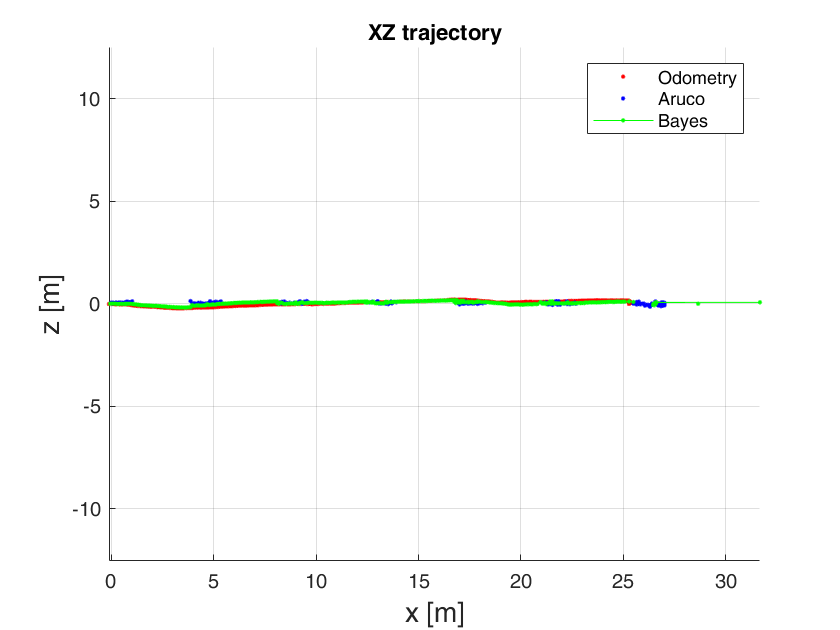
\includegraphics[width=.4\textwidth]{images/bayesexpaxeq.png}
        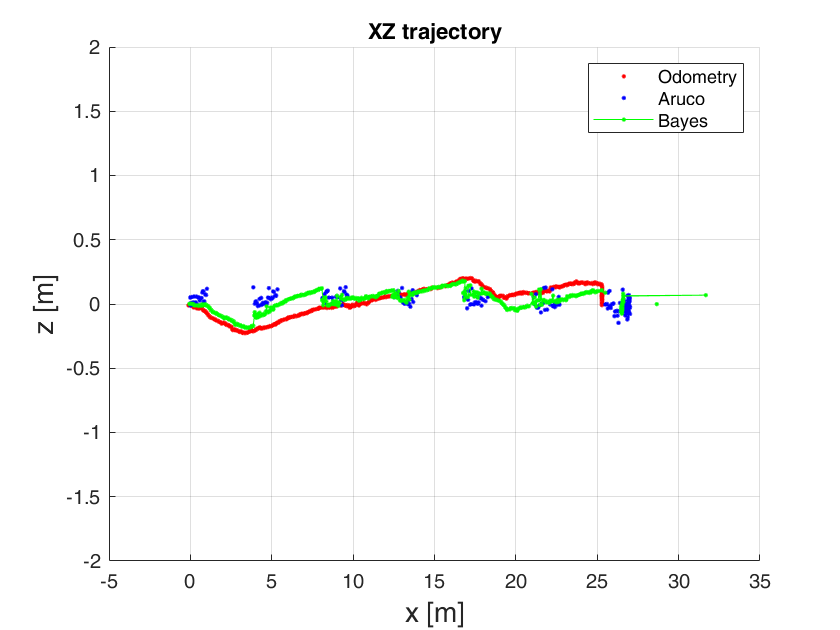
\includegraphics[width=.4\textwidth]{images/bayesexp.png}
        \caption{Grafico dei risultati della fusione, su due scale differenti.}
    \end{figure}
\end{frame}

\begin{frame}{Algoritmi di sensor fusion}
\framesubtitle{Teorema di Bayes-risultati}
    \begin{figure}
        \centering
        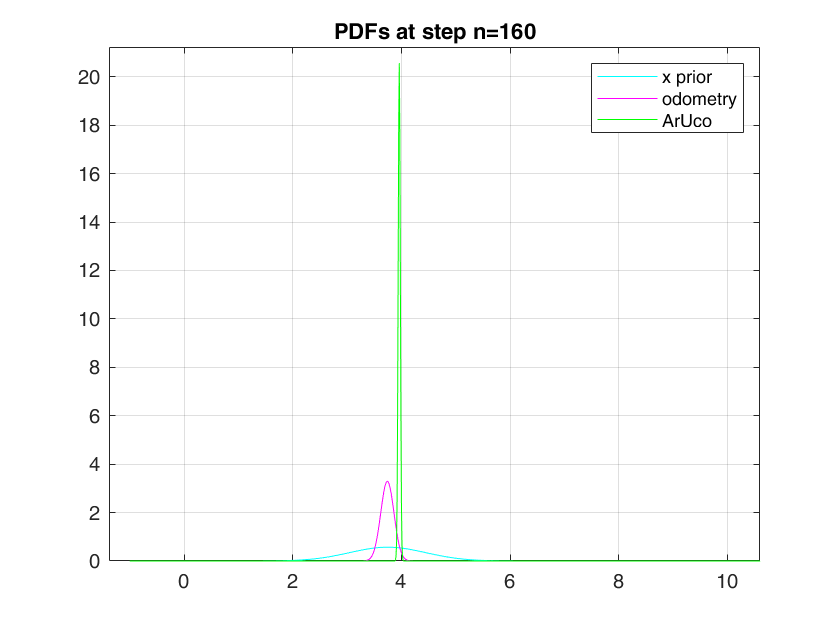
\includegraphics[width=.4\textwidth]{images/pdfs.png}
        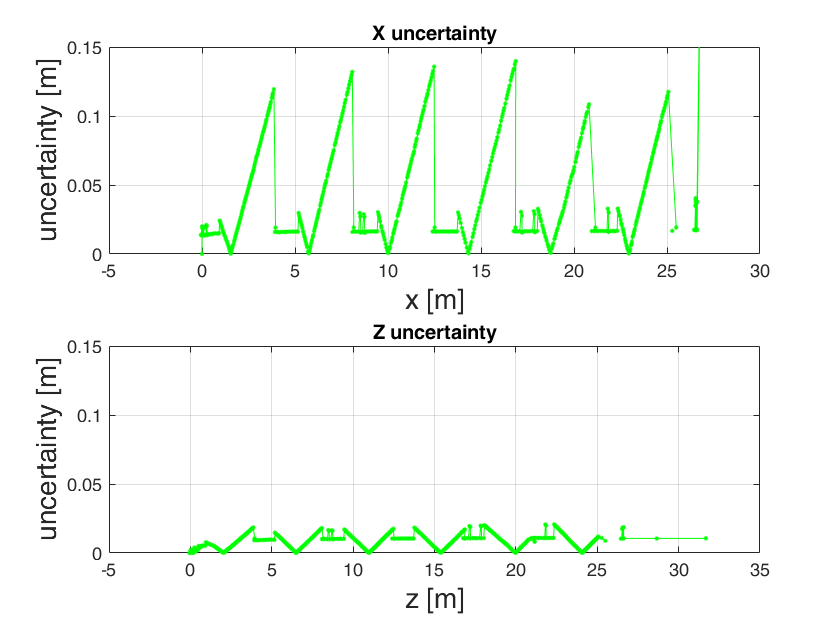
\includegraphics[width=.4\textwidth]{images/fuseduncBayes.png}
        \caption{Esempio di pdf (sinistra) e andamento dell'incertezza di misura (a destra).}
    \end{figure}
\end{frame}

\begin{frame}{Algoritmi di sensor fusion}
\framesubtitle{Conclusioni}
\begin{table}[h]
    \centering
    \begin{tabular}{|c|c|c|c|c|}
    \hline
        Algoritmo &  odometria & clt & kf & Bayes\footnote{Sono state escluse le misurazioni dove le misurazioni erano incompatibili per la fusione} \\
        \hline
        rmse X [m] & $8.9$ & $1.1$ & $1.2$ & $0.56$ \\
        \hline
        rmse Z [m] & $0.096$ & $0.068$ & $0.080$ & $0.068$\\
        \hline
    \end{tabular}
    \caption{Confronto tra rmse ottenuti dall'odometria e dagli algoritmi utilizzati}
\end{table}
    
\end{frame}

\end{document}
